\chapter{Background \& Objectives}


\section{Background}
In this section I will be talking about the Wizard Card Game, how the game works and how you can win the game and show in the this video\cite{wizardVideo}. I will also discuss the Artificial Intelligence techniques that were consider using for the opponents, which are neural networks, minmax and Monte Carlo algorithms. This will be expanded upon to how I concluded using the Monte Carlo Tree search for this game.
\subsection{Wizard Card Game}
\subsubsection{Dealing and Setup}
Wizard is a card game that contains 52 normal deck cards and 8 extra cards 4 of which are called wizards and the other 4 are called jesters\cite{wizardOver}.  Each player is dealt the same number of cards that is the round. For example, round 1 means each person get 1 card but round 10 means they each get ten cards. This is then played until the is no cards left to be dealt out mean for 3 people there should be 20 round and 15 rounds for 4 people. A trump card is also dealt from the deck at the beginning of the round from the top.  After each play in a round the dealer is changed clockwise.
\subsubsection{Playing and Bidding}
One the trump has been dealt, the person to the left of the dealer states how many tricks they think they will win in this round. The maximum they can bid it the number of cards they have in their hands.  Once everyone has put their individual bids in, the player to the left of the dealer puts down the first card which can be any card they want, then each player can either match the suit that the first player put down or the better play it to match the trump suit or play a wizard to win. Otherwise they can play off suit or play a jester to lose.
\subsubsection{Scoring}
To score points in this game you must use the bid on how many tricks you think you can win, giving you 20 point for being right and 10 point for every trick you win. Otherwise you get negative 10 point per every trick you were over or under for that round. For example, if you guess 4 tricks to win and only one 1 you would lose 30 points. 

\subsection {Monte Carlo Alogrithm}
The Monte Carlo Algorithm is probilistic search alogrithm that creates a tree based on the current states of the problem. This is then randomly expanded from the root node and simulated what might happen, under specfic constrains such a iterations of the simulation or under an amount time. This will then gvie a score back on what how well the simulation wen. once this is done the best option will be picked based on what has the higest score from the tree that has currently been created.  The next sections belows wil show the 4 phases that are used in the algorithm.
\begin{figure}[h]
\centering
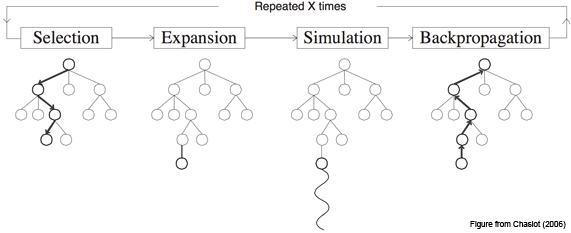
\includegraphics[width=15cm]{mcts-algorithm-1a}
\caption{Diagram Showing Steps in Monte Carlo Tree Search}
\end{figure}[h]
\subsubsection{Selection}
For this plase in the algorithms it will start with the root node that shows the intial state of the game. This will then select the child node that has the best win rating. this win rating will be selected by the use if Uct(Upper Confindence Bound for Trees). The formula used for this is:
\begin{figure}[h]
\centering
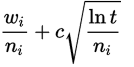
\includegraphics[width=5cm]{formula}
\caption{Shows the UCT formula}
\end{figure}[h]

\begin{itemize}
\item w\textsubscript{i} : This variable will contain the number of wins the node will have after \textit{i} amount of moves.
\item n\textsubscript{i} : This is the number of simulation after the \textit{i} amount of moves
\item c : This is this exploration parameter and should theoretically be equal to .
\item t : the total number of simulations performs for the parent node.
\cite{mctswithcode}
\end{itemize}
\subsubsection{Expansion}
After the selection of a node is complete we do the expansion of this node. This is done by adding a new child node to the tree that was optimally reached during the selection process\cite{mctsSource}.
\subsubsection{Simulation}
Once the  node has been expanded ,we perform a simulation of the state until it reach the end of what we are trying to achieve. For example in  the project we would simulate the selection of the cards until there are non left and how large there score is.
\subsubsection{Backpropagation}
In this part of the process we look at the result of the simulation and give a rewards for how good the simualation was. In the context of this game the close the score is to the intial bid the better it is, meaning that we shall reward the child node with a higher score the larger the score and closer to the bid.


Once this is done under it will be repeat for a set number of iterations or under a specific time peroid. This will then create an asymmetric search tree that grows after each iterations through the steps. Once it is done iterating, it will pick the best child node best on the best score divided by the amount of visits that specific node has.
\subsubsection{Advantages}
\begin{itemize}
\item Compared to other Ai alogrithms this is quite a simple algorithm to implement.
\item As this is a huristic alogirthm is does not need to everything that happens in the game apart from the rules of the game, how it ends the simulation/leaf node and what cards the player may have. this is beacause it can find it own moves and randomly playout the game.
\item The tree that has been creates can be used for the future meaning less computational expense creating more nodes.
\item As you can select the number of iterations/time given, it means you can make the tree as small or large as you would like. 
\end{itemize}
\subsubsection{Disadvantages}
\begin{itemize}
\item Tthe larger the tree growths the more rapidly memory expensive.
\item The algorithm normally needs a large amount of iteration to be able to effectively pick the best path ,meaning that it will have to take amount of time to construct a large enough search space.
\end{itemize}

\subsection{Similar Algorithms}
In this section, I will be talking abolu the two other Algorithms that could of been used for the Artifical intelligence of the game. I will also discuss why they werent used and why the Monte Carlo Tree Search was the one i picked.
\subsubsection{Neural Network}
Neural Network are artifically created based on the neuronal structure of the mamalian cerebral cortex but on much smaller scales.\cite{NeuralNetwork}
\subsubsection{MinMax}


\section{Analysis}
In this section I will be talking about what I will be aiming doing achieve with this product and what technology I will be using during this process. 
\subsection{Project Aims}
The aim for this project is create a functional software version of the card game Wizard. This will also contain an Artifical intelligence Opponent that uses the Monte Carlo Algorithm to select a card for that round. The game will be simplified to only have 3 players, two of whihc will be the AI and one which is the human player. Each player will have 15 cards each and play until there are no cards left for 5 rounds. 
\subsection {Technology Overview}
\subsubsection{Programming Language}
Use Java
\subsubsection{Hardware}
Say Specifiction of Harware used, and not need be helpful for faster processing speed.
\section{Research Method and Software Process}
\subsection {Foreseen Challenges}
applying Rules, Implementiong MonteCarlo Tree search and optimising.
\subsection {Process Methodology}
There was a lot of options for developing my project. In the end I decide to you a agile approach based on Scrum. This would give me an iterative way of progressing in the project, use the sprints in the methodology to progressively improve on the previous work that I have done, adding more functionality and complexity to it as it is being developed.I feel this was a better option that a traditional process such as the waterfall model. This is because I can start work on the software whilst writing up the report without having to do redo all the work I have previously done when changes are made to the design of the software.
\subsubsection{Version Control}


